\chapter{Конструкторская часть}

\section{Функциональная схема работы программы}

На рисунках \ref{fig:idef0} и \ref{fig:idef0a0} представлена функциональная схема работы программы.

\begin{figure}[h!]
	\centering
	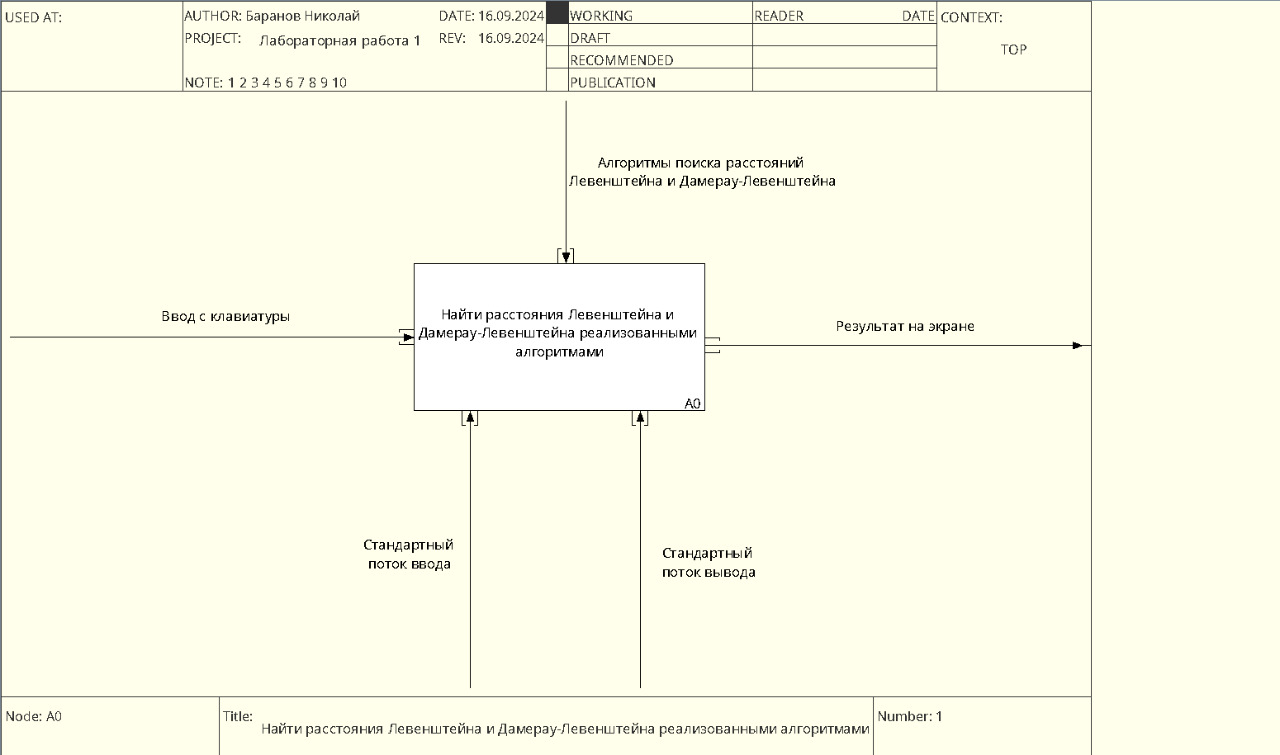
\includegraphics[width=0.8\textwidth]{tex_parts/idef0.png}
	\caption{\label{fig:idef0}Верхний уровень функциональной схемы}
\end{figure}

\begin{figure}[h!]
	\centering
	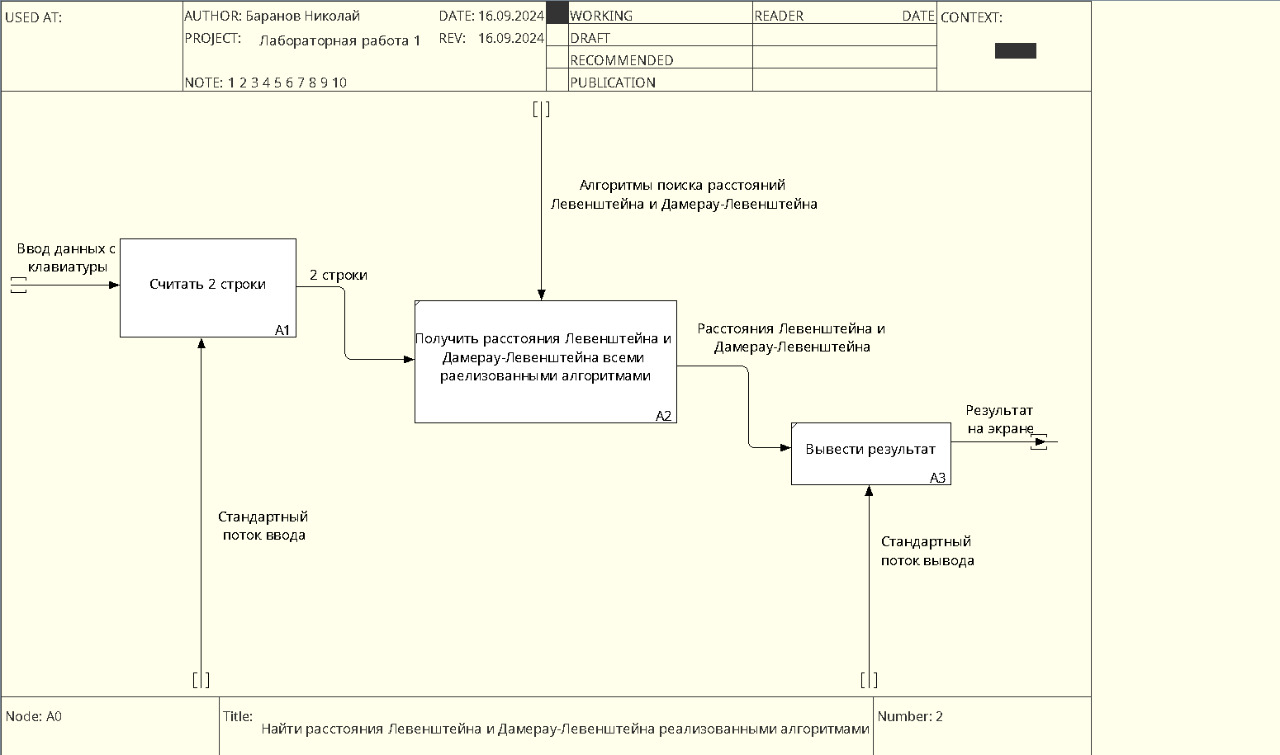
\includegraphics[width=0.8\textwidth]{tex_parts/idef0a0.png}
	\caption{\label{fig:idef0a0}Декомпозиция уровня A0}
\end{figure}

\section{Схемы алгоритмов}

На вход каждому из алгоритмов подаются строки first и second длиной n и m соответственно. Алгоритм с мемоизацией также будет получать матрицу cache размером n+1 на m+1.

\begin{figure}[h!]
	\centering
	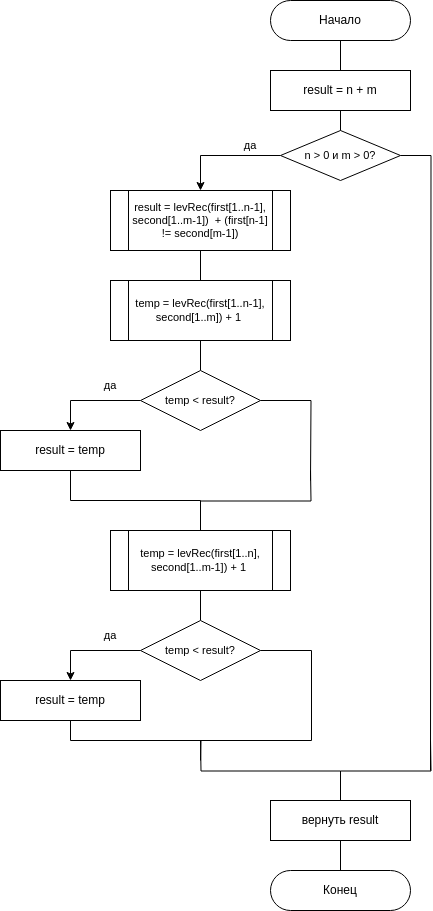
\includegraphics[height=0.7\textheight]{tex_parts/scheme1.png}
	\caption{\label{fig:levRec}Схема рекурсивного алгоритма нахождения расстояния Левенштейна}
\end{figure}

\clearpage

\begin{figure}[h!]
	\centering
	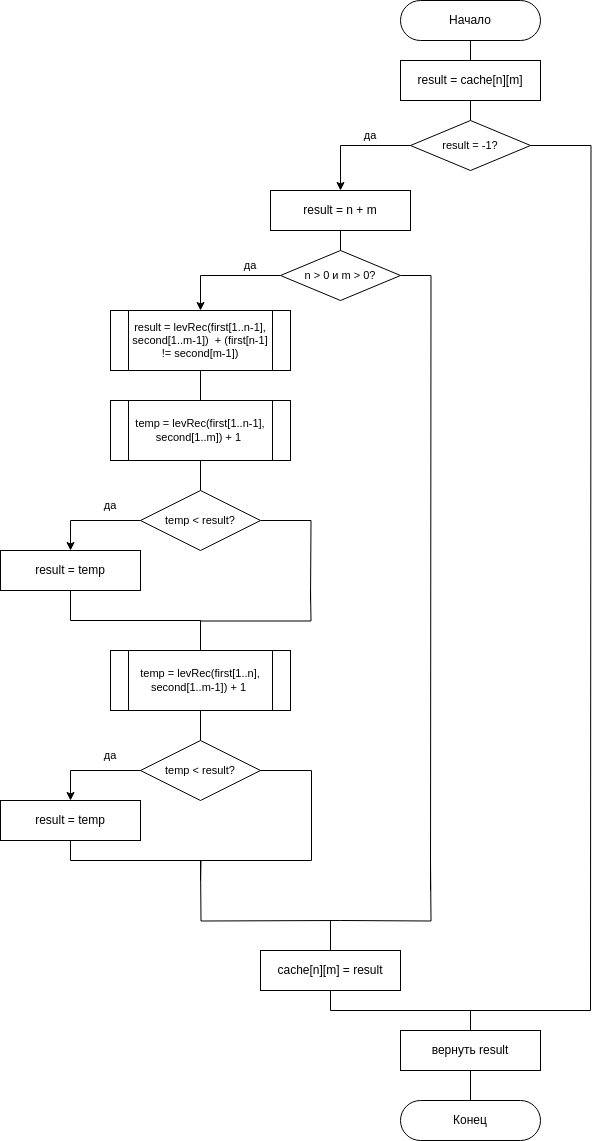
\includegraphics[height=0.8\textheight]{tex_parts/scheme2.png}
	\caption{\label{fig:levMem}Схема рекурсивного алгоритма нахождения расстояния Левенштейна с мемоизацией}
\end{figure}

\clearpage

\begin{figure}[h!]
	\centering
	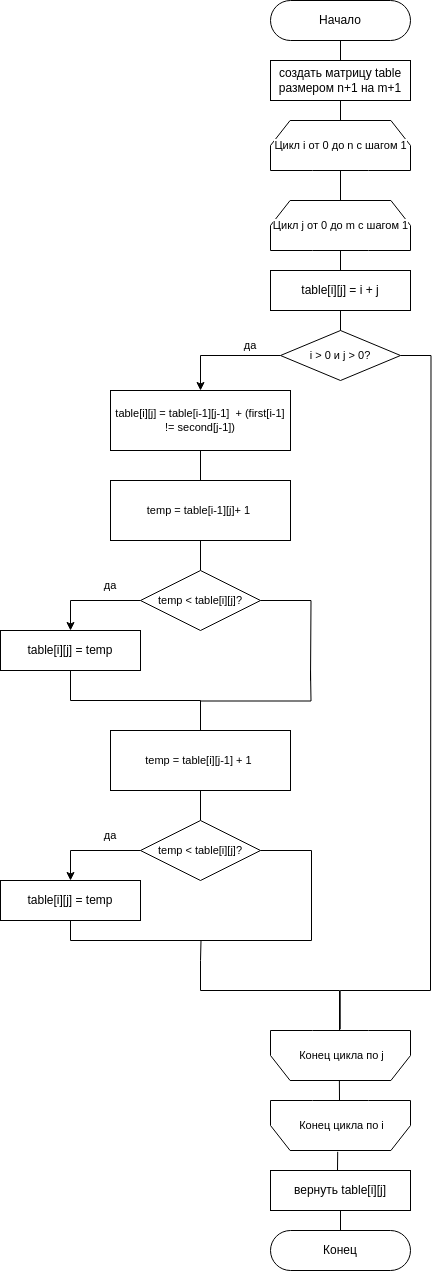
\includegraphics[height=0.8\textheight]{tex_parts/scheme3.png}
	\caption{\label{fig:levItr}Схема матричного алгоритма нахождения расстояния Левенштейна}
\end{figure}

\clearpage

\begin{figure}[h!]
	\centering
	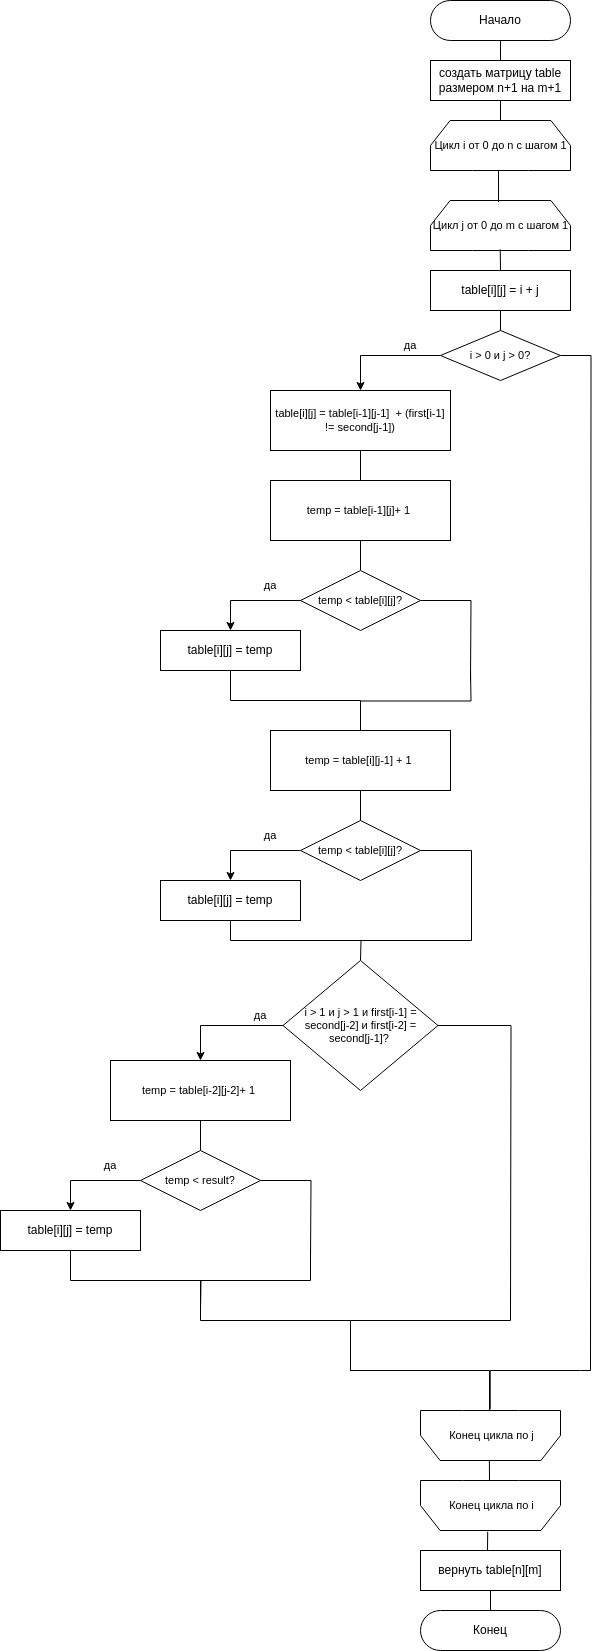
\includegraphics[height=0.8\textheight]{tex_parts/scheme4.png}
	\caption{\label{fig:damItr}Схема матричного алгоритма нахождения расстояния Дамерау-Левенштейна}
\end{figure}

\clearpage

\section{Используемые типы и структуры данных}

При реализации алгоритмов будут использованы следующие структуры данных:

\begin{itemize}
	\item строка --- массив символов;
	\item длина строки --- целое беззнаковое число;
	\item матрица --- двумерный массив целых беззнаковых чисел.
\end{itemize}

\section{Выводы}

В данном разделе была представлена функциональная схема работы программы, а также были построены схемы алгоритмов и выбраны структуры данных.

